% 1991 年上海卷第 26 题：过定点 A(2,0) 的动直线 L 与抛物线 y=x^2+2 交于 B、C（依固定扫描页重绘，只画拓扑与标号，不按比例）
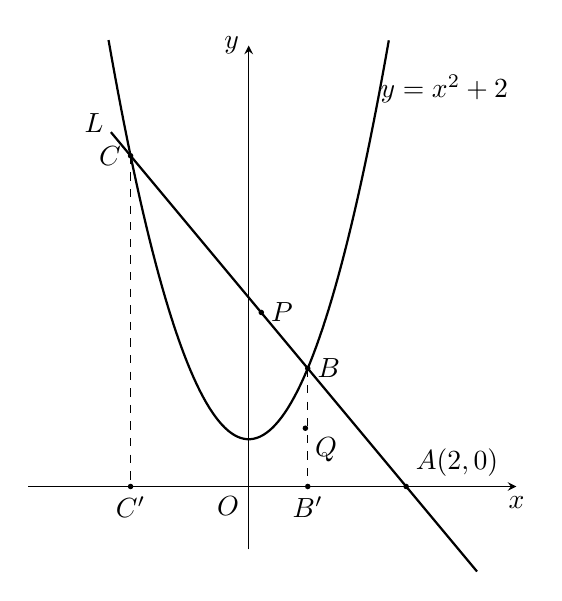
\begin{tikzpicture}[>=stealth,scale=1.0]
  % 坐标轴
  \draw[->] (-2.8,0)--(3.4,0) node[below] {$x$};
  \draw[->] (0,-0.8)--(0,5.6) node[left] {$y$};
  \node[below left] at (0,0) {$O$};
  % 抛物线（示意，非按比例）
  \draw[thick,domain=-1.78:1.78,samples=90] plot (\x,{1.6*(\x)^2+0.6});
  \node[right] at (1.55,5.05) {$y=x^{2}+2$};
  % 动直线 L（过 A(2,0)）
  \draw[thick] (-1.75,4.50)--(2.9,-1.08) ;
  \node[left] at (-1.72,4.62) {$L$};
  % 交点与射影
  \coordinate (C) at (-1.50,4.20);
  \coordinate (B) at (0.75,1.50);
  \coordinate (Cp) at (-1.50,0);
  \coordinate (Bp) at (0.75,0);
  \coordinate (A) at (2,0);
  \coordinate (P) at (0.16,2.21);
  \coordinate (Q) at (0.72,0.74);
  \draw[dashed] (C)--(Cp);
  \draw[dashed] (B)--(Bp);
  \fill (C) circle (1pt) node[left] {$C$};
  \fill (B) circle (1pt) node[right] {$B$};
  \fill (Cp) circle (1pt) node[below] {$C'$};
  \fill (Bp) circle (1pt) node[below] {$B'$};
  \fill (A) circle (1pt) node[above right] {$A(2,0)$};
  \fill (P) circle (1pt) node[right] {$P$};
  \fill (Q) circle (1pt) node[below right] {$Q$};
\end{tikzpicture}
